\section{Introduction}

    \subparagraph{}Le but de ce {\color{info}5\ieme{} travail} est de réaliser un circuit avec au minimum 5 résistances,
    une source de tension et de courant, une inductance et un interrupteur qui se ferme ou s'ouvre en $t\; =\; 0$ et enfin
    de simuler le circuit avec le logiciel \textit{LTspice} afin de démontrer l'exactitude des calculs.\\[1.5cm]
    
    \begin{titletbox}{À l'attention du correcteur / correctrice}{warning}
        N'hésitez pas à zoomer sur les schémas du circuit et autres images afin d'y voir plus clair.
    \end{titletbox}

\section{Schéma initial du circuit}

    \begin{figure}[H]
        \centering
        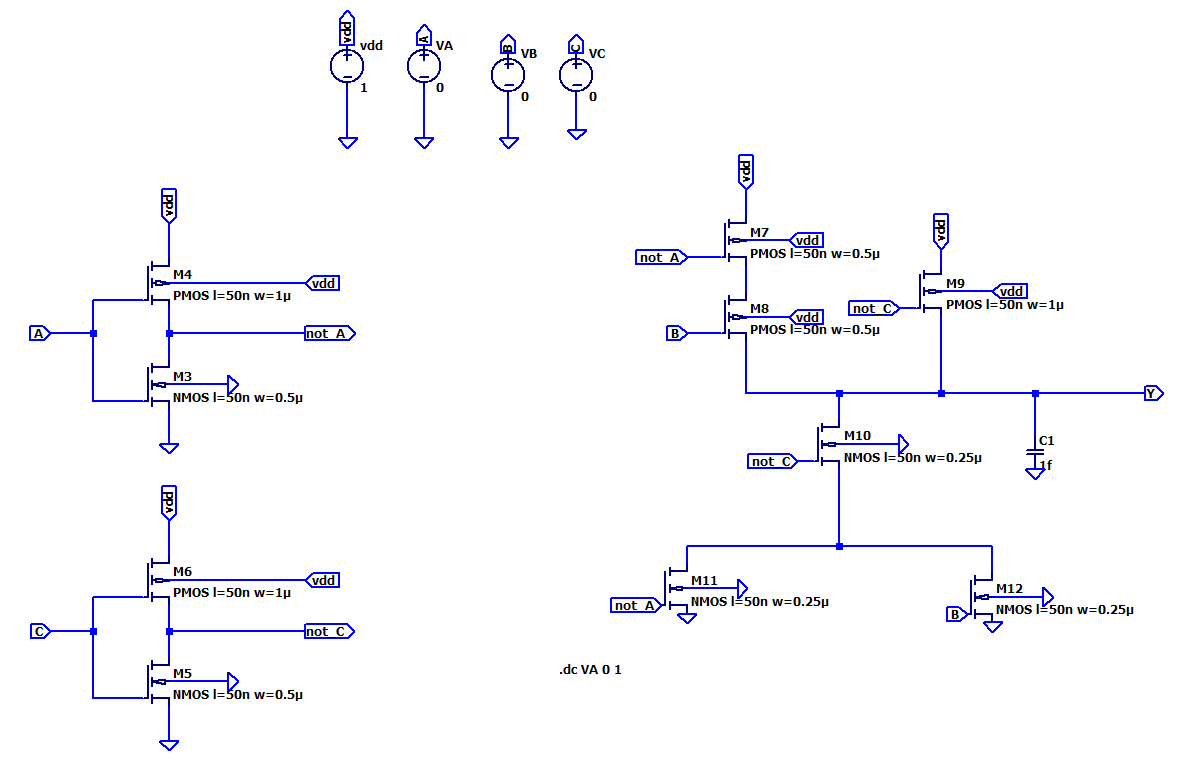
\includegraphics[scale=0.5]{../pictures/circuit.png} % Pas utiliser width=\textwidth pcq il prend la taille de \section{} comme ref
        \caption{Schéma du circuit}
    \end{figure}

    \section{Calcul de la condition initiale : $I_L(t\leq0)$}

    \subparagraph{}L'interrupteur étant ouvert en $t\leq0$ et l'inductance se comportant comme un court-circuit, j'obtiens le morceau suivant :
    
        \begin{figure}[H]
            \centering
            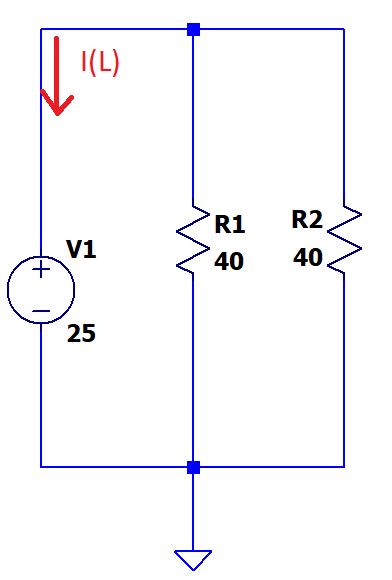
\includegraphics[width=0.3\textwidth]{../pictures/open.PNG}
            \caption{Circuit en condition initiale}
        \end{figure}
        
        
    \subparagraph{} On peut mettre $R_1$ et $R_2$ en // ce qui nous donne une résistance équivalente de 20 $\Omega$. Avec ceci, on peut calculer le courant grâce à la formule suivante :
    
        {\color{info}\begin{align*}
            I_L(t)\;&=\;-\frac{V}{R}\\
            I_L(t)\;&=\;-\frac{25}{20}\\
        \end{align*}}
    
    \begin{empheq}[box=\fbox]{equation*}
    \color{red}
        I_L (t\leq0)\;=-\;1,25\;A
    \end{empheq}

\section{Calcul de la condition finale : $I_L(t=\infty)$}
    
    \subparagraph{}En condition finale, l'interrupteur est fermé et nous avons donc le circuit suivant :
    
        \begin{figure}[H]
            \centering
            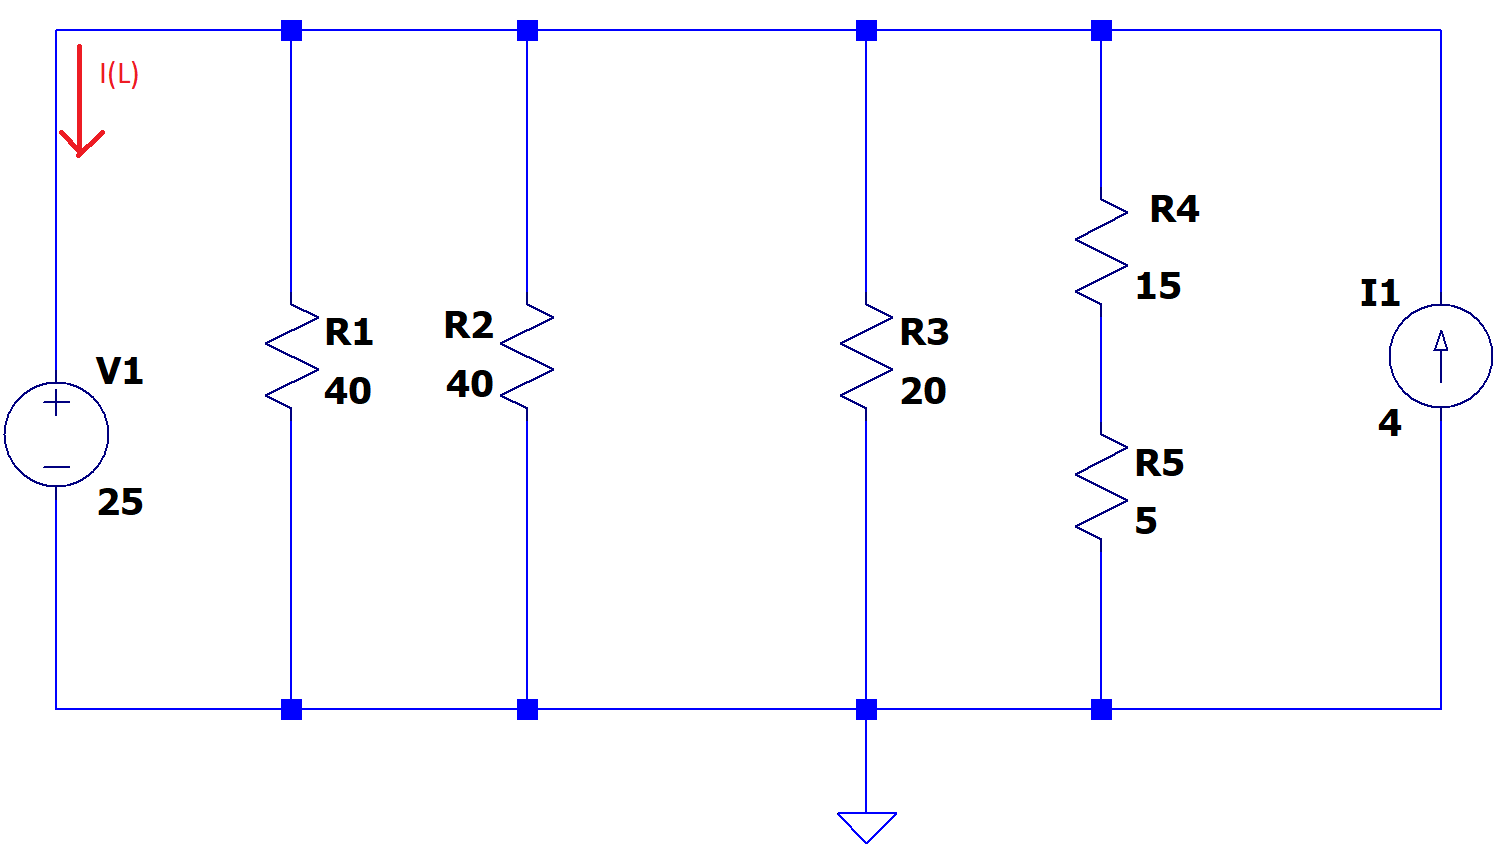
\includegraphics[width=0.7\textwidth]{../pictures/close.PNG}
            \caption{Circuit en condition finale}
            \label{fig:final}
        \end{figure}
        
    \subparagraph{}On peut simplifier le circuit comme tel :
        
        {\color{info}\begin{align*}
            R_{eq}\;&=\;(R_1 // R_2) // R_3 // (R_4 + R_5)\\
            R_{eq}\;&=\;(40 // 40) // 20 // (15 + 5)\\
            R_{eq}\;&=\;\frac{20}{3}\;\Omega\\
        \end{align*}}
        
        
        
    \subparagraph{}Grâce à la loi des noeuds, nous pouvons poser l'équation suivante pour trouver $I_L$ :
    
        {\color{info}\begin{align*}
            4\;=&\;I_L + \frac{25}{\frac{20}{3}} \\
            4 - 3.75\;=&\;I_L\\
            0.25\;=&\;I_L\\
        \end{align*}}
        
    \subparagraph{}On obtient donc :
        \begin{empheq}[box=\fbox]{equation*}
            \color{red}
                I_L (t=\infty)\;=\;0.25\;A
        \end{empheq}
        


\section{Calcul de la constante de temps $\tau$}

    \subparagraph{}La constante $\tau$ peut se calculer via la formule suivant :
    
        \begin{equation*}
            \color{info}
            \tau\;=\;\frac{L}{R}
        \end{equation*}
        
    
    \subparagraph{}On peut donc  calculer $\tau$ :
    
        {\color{info}\begin{align*}
            \tau\;&=\;\frac{100n}{\frac{20}{3}} \\
            \tau\;&=\;15\;nS \\
        \end{align*}}
        
        \begin{empheq}[box=\fbox]{equation*}
            \color{red}
            \tau\;=\;15\;nS
        \end{empheq}

\section{Courant de l'inductance $I_L(t)$ pour $t>0$}

    \subparagraph{}On peut calculer la tension suivant la formule suivante :
    
        {\color{info}\begin{align*}
            I_L(t)\;&= A + B \cdot \euler^{\frac{-t}{\tau}} \\
            I_L(t)\;&= I_{\infty} + (I_0 - I_{\infty}) \cdot \euler^{\frac{-t}{\tau}} \\
            I_L(t)\;&= 0.25 + (-1.25 - 0.25) \cdot \euler^{\frac{-t}{15\;nS}} \\
            I_L(t)\;&= 0.25 - 1.5\cdot \euler^{\frac{-t}{15\;nS}} \\
        \end{align*}}
        
        \begin{empheq}[box=\fbox]{equation*}
            \color{red}
            I_L(t)\;= 0.25 - 1.5\cdot \euler^{\frac{-t}{15\;nS}}\;A
        \end{empheq}
        
\section{Tension aux bornes de l'inductance $V_L(t)$ pour $t>0$}
        
    \subparagraph{}On peut calculer le courant de l'inductance suivant la formule suivante :
        {\color{info}\begin{align*}
            V_L(t)\;&=\;L \cdot \frac{dI_L}{dt}\\
        \end{align*}}
        
    \subparagraph{}En résolvant la dérivée, on obtient ({\color{info}$G$} signifie giga) :
    
         {\color{info}\begin{align*}
            V_L(t)\;&=\;L \cdot \frac{1}{10}G \cdot \euler^{\frac{-t}{15\;nS}}\\
            V_L(t)\;&=\;100n \cdot \frac{1}{10}G \cdot \euler^{\frac{-t}{15\;nS}}\\
        \end{align*}}
        
        \begin{empheq}[box=\fbox]{equation*}
            \color{red}
            V_L(t)\;=\;10 \cdot \euler^{\frac{-t}{15\;nS}}\;V
        \end{empheq}
        
\section{Simulation du circuit}
        \begin{figure}[H]
            \centering
            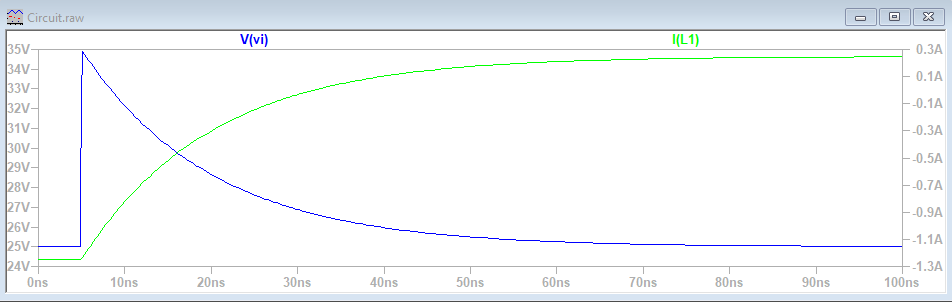
\includegraphics[width=0.9\textwidth]{../pictures/simu.png}
            \caption{Simulation du circuit, avec la tension en bleu et le courant en vert}
        \end{figure}
\section{Conclusion}

    \subparagraph{}En conclusion, on remarque qu'en condition initiale j'ai bien -1.25 A et 0.25 A en condition finale ce qui confirme mes calculs. (voir \textbf{Figure 5} ci dessous) Le délai de 4 nanosecondes dans mon graphique s'explique par le fait que j'ai mis un délai dans ma commande PULSE sur $LTspice$.
    
    \begin{figure}[H]
            \centering
            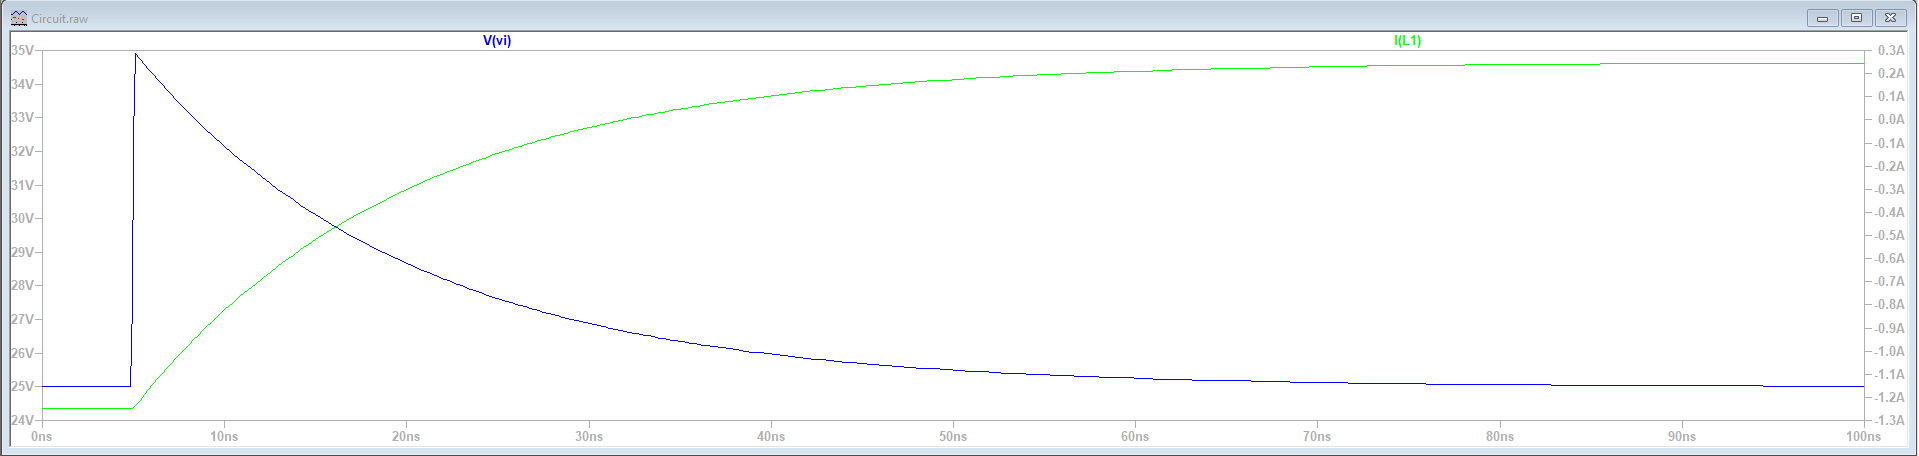
\includegraphics[width=\textwidth, angle=90]{../pictures/zoom.PNG}
            \caption{Résultats de la simulation zoomée}
    \end{figure}

\end{document}